\documentclass[tikz,border=4pt]{standalone}
\usetikzlibrary{arrows.meta}
\begin{document}
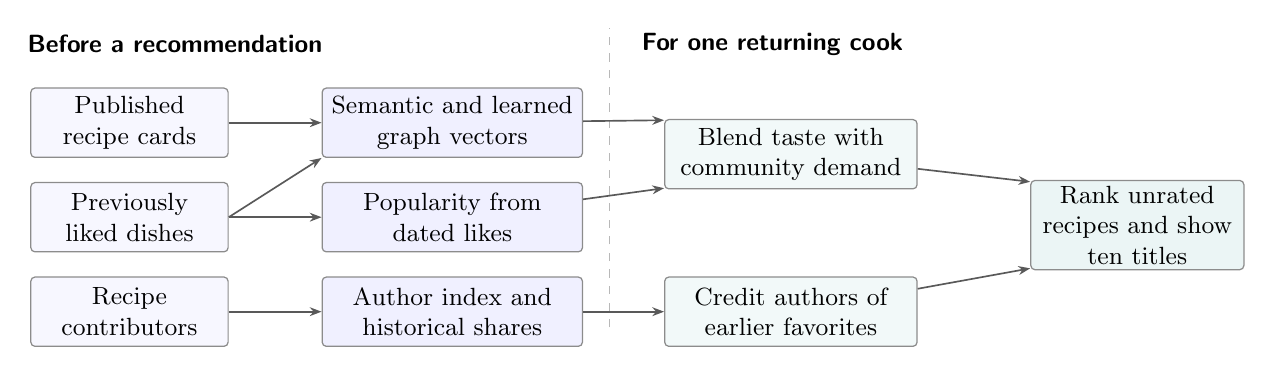
\begin{tikzpicture}[x=1mm,y=1mm,
  stage/.style={draw=black!45,rounded corners=1.5pt,line width=.45pt,align=center,font=\small,inner xsep=1.5pt,inner ysep=2pt,minimum height=8.8mm},
  label/.style={font=\small\sffamily\bfseries,anchor=west,inner sep=0pt},
  flow/.style={-{Stealth[length=1.5mm]},line width=.6pt,draw=black!65}]
  \node[label] at (0,36) {Before a recommendation};
  \node[label] at (78,36) {For one returning cook};
  \draw[black!28,dashed] (74,0) -- (74,38);
  \node[stage,fill=blue!3,text width=24mm] (cards) at (13,26) {Published\\recipe cards};
  \node[stage,fill=blue!3,text width=24mm] (likes) at (13,14) {Previously\\liked dishes};
  \node[stage,fill=blue!3,text width=24mm] (byline) at (13,2) {Recipe\\contributors};
  \node[stage,fill=blue!6,text width=32mm] (graph) at (54,26) {Semantic and learned\\graph vectors};
  \node[stage,fill=blue!6,text width=32mm] (pop) at (54,14) {Popularity from\\dated likes};
  \node[stage,fill=blue!6,text width=32mm] (author) at (54,2) {Author index and\\historical shares};
  \node[stage,fill=teal!5,text width=31mm] (taste) at (97,22) {Blend taste with\\community demand};
  \node[stage,fill=teal!5,text width=31mm] (familiar) at (97,2) {Credit authors of\\earlier favorites};
  \node[stage,fill=teal!8,text width=26mm] (rank) at (141,13) {Rank unrated\\recipes and show\\ten titles};
  \draw[flow] (cards) -- (graph);
  \draw[flow] (likes.east) -- (graph.south west);
  \draw[flow] (likes) -- (pop);
  \draw[flow] (byline) -- (author);
  \draw[flow] (graph) -- (taste.165);
  \draw[flow] (pop) -- (taste.195);
  \draw[flow] (author) -- (familiar);
  \draw[flow] (taste) -- (rank.158);
  \draw[flow] (familiar) -- (rank.202);
\end{tikzpicture}
\end{document}
